\documentclass[paper=a4,10pt]{scrartcl}

\usepackage[utf8x]{inputenc}
\usepackage[ngerman]{babel}
\usepackage[T1]{fontenc}

\usepackage{graphicx}
\usepackage{float}
\usepackage{subcaption}

\usepackage{fancyref}

\usepackage[numbers,square,sort]{natbib} %praktikumsquellenvorgabe
\usepackage{amsmath}
\usepackage{amssymb}

\usepackage{url}
\usepackage{hyperref}

\usepackage[a4paper, includehead, includefoot]{geometry}
\geometry{left=2cm, right=2cm, top=2cm, bottom=2cm}

\begin{document}

\title{Ma-Notizen}
%\author{Author's Name}

\section{Todo}
\begin{itemize}
\item graphical models
\item BP, SP
\item Bethe approx
\item Verbindung zwischen den ersten beiden Punkten
\item Max-Sum
\item integrality gap
\item (conditional value at risk)
\item Kruskal Alg.
\end{itemize}

\section{s-t-path, kürzester Pfad}
Pfad zwischen zwei Knoten $s, t\in V$ eines Graphen, welcher minimale Länge bzgl. einer Kostenfunktion $c: E \rightarrow \mathbb{R}$ hat.

\section{Cut}
Ein Cut $C=(S,T)$ ist eine partition von $V$ eines Graphen in die zwei disjunkten Subsets $S$ und $T$.
Als cut-set eines Cuts bezeichnet man die Menge der Kanten die einen Endpunkt in $S$ und den anderen in $T$ haben: $E' = \{ \{i,j\} \in E \ | \ i \in S, j \in T\}$. Und man sagt, eine Kante ist im Cut, wenn sie Element von $E'$ ist.

\section{Tree Cut}
Wenn man einen Spannbaum hat und eine Kante daraus entfernt, kann man sagen, dass dadurch einen Cut entsteht.

\textit{Dadurch dass man eine Kante weglässt, bleiben zwei Komponenten übrig und deren Knotenmengen sind dann die Cutmengen.} 

\section{Minimum spanning tree equivalente Formulierungen}
\subsection{path optimality condition}
Ein Spannbaum ist dann ein minimum Spannbaum von einem connected Graph if and only if it satisfies the path optimality condition:
Für jede nontree Kante $\{i, j\}$ von $G$ gilt $w_{i,j} \ge w_{u,v}$ für alle Kanten $\{u, v\}$ im tree path $P_{i,j}$ der im Spannbaum die Knoten $i$ und $j$ verbindet.
\textit{Wenn das nicht so wäre, könnte man einen neuen Spannbaum erzeugen, bei dem ich eine Kante mit größeren Kosten aus dem tree path durch die Kante $\{i,j\}$ ersetze und hätte so geringere Kosten, also kann der Ausgangsspannbaum nicht minimal gewesen sein.}
\subsection{cut optimality condition}
Ein Spannbaum ist dann MST von connected Graph $G$ if and only if it satisfies the cut optimality condition:
Für jede tree Kante $\{i, j\}$ von $G$ gilt $w_{i,j} \le w_{u,v}$ für alle Kanten $\{u, v\}$ die im Cut sind, den man durch Entfernen von $\{i, j\}$ erhält.

\textit{Mit 'im Cut sind' ist die Formulierung von oben gemeint. Die Aussage ist also die, wenn ich nen MST habe, dann kann ich wenn ich eine Kante daraus nehme und damit einen Cut erzeuge keine andere Kante finden mit der ich eine Brücke zwischen den Cutkomponenten bauen könnte, die ein geringeres Gewicht als die entfernte Kante hat.(fuer die alternative Kante werden Kanten in Betracht gezogen, die nicht Teil des geg. Spannbaums sind, sondern welche, die auch in dem erzeugten Cut sind.)}

\section{Minmax spanning tree Problem}
Im Paper Ontheapproximabilityofrobustspanningtreeproblems wurde ich zum ersten Mal auf diese Problemstellung aufmerksam. Es geht erstmal um das ein stage Problem des minimalen Spannbaumes mit uncertain (nicht im Sinne von Lius uncertain variables) edge weights. Es geht hier um das robust optimization setting, bei welchem alle möglichen Gewichtsrealisierungen als Szenarien aufgelistet werden, es allerdings darauf keine Wahrscheinlichkeitsverteilung gibt. Das minmax Kriterium ist nun dazu da, um trotzdem eine Entscheidung zu treffen. Sei $\phi$ die Menge aller Spannbäume des connected Graphen $G$, $\Gamma=(S_1, \dots, S_k)$ die Menge aller Szenarien (Kostenrealisierungen) und wir befinden uns im unbounded case, wo die Anzahl von Szenarien Teil des Inputs ist. Das minmax spanning tree problem ist nun so formuliert:
\begin{align}
\text{OPT} = \min_{T \in \phi} \max_{S \in \Gamma} \sum_{e \in T} c_e^S
\end{align}
\textit{Ich verstehe das so: Wir suchen also von allen Spannbäumen auf dem Graphen $G$ denjenigen $T$, für den der schlimmste Wert der Kosten am kleinsten ist. Wenn ich einen anderen Spannbaum nehmen würde, dann gibt es mindestens ein Szenario, bei welchem die Kosten größer werden würden, als sie es hier maximal werden können.}
In dem Paper wird außerdem eine minmax Version für das two stage spanning tree problem beschrieben.

\section{Matching}
\subsection{Definition}
Sei $G=(V,E)$ ein endlicher, ungerichteter Graph. Eine Menge $M\subseteq E$ ist ein Matching, wenn es keine zwei Kanten in $M$ gibt, welche inzident zum selben Knoten sind, also den selben Knoten enthalten.

\paragraph{maximal matching}
Ein Matching $M$ heißt maximal matching (nicht erweiterbar), wenn es keine weitere Kante $e \in E \setminus M$ gibt für welche $\{ e\} \cup M$ eine weiteres gültiges Matching wäre.

\paragraph{maximum matching}
$M$ heißt maximum matching (größtmögliches Matching), falls $M$ von allen möglichen Matchings die größte Kardinalität aufweist. Maximum matchings sind auch maximale Matchings und die Mächtigkeit eines Maximum matchings wird Matchingzahl genannt und als $\nu(G)$ notiert.

\paragraph{perfekte matchings}
$M$ ist perfekt, wenn $2 \cdot |M| = V$ gilt, also jeder Knoten des Grapheneinmal in den Kanten in $M$ vorkommen. Perfekte Matchings sind maximum matchings und damit auch maximal. 

\subsection{Eigenschaften}
Seien $A$ und $B$ zwei maximale matchings. 

\begin{itemize}
\item Jede Kante in $B \setminus A$ kann höchstens mit zwei Kanten in $A \setminus B$ benachbart sein (Kanten nennt man benachbart, wenn sie einen Knoten teilen). \\
\textit{Eine Kante, die in $B \setminus A$, also in $B$, aber nicht in $A$ vorkommt hat nur zwei Knoten und da $A$ ein Matching ist, kann es in $A$ nur maximal zwei Kanten geben, die inzident zu diesen Knoten sind (entweder zwei Kanten von denen jeweils eine inzident zu eine der beiden Knoten ist, oder nur einer der Knoten ist von $A$ abgedeckt). Da es also nur maximal zwei Kanten in $A$ geben kann, welche mit einer Kante in $B \setminus A$ benachbart sein können, gilt dies auch für $A \setminus B$ (die Menge wird dadurch ja nur kleiner, aber das gilt schon für die Große).}

\item Jede Kante in $A \setminus B$ grenzt an (mindestens?) eine Kante in $B \setminus A$, weil $B$ nicht erweiterbar ist.\\
\textit{Eine Kante, die in $A \setminus B$ vorkommt, hat wieder zwei Knoten $v, w$. Es kann nicht sein, dass keiner von den beiden Knoten in einer Kante in $B$ vorkommt, weil sonst könnte man $B$ um die Kante $\{v, w\}$ erweitern, was aber per Definition nicht möglich ist. Also werden entweder beide oder nur einer in Kanten von $B$ berücksichtigt. So oder so ist mindestens ein Knoten in einer Kante in $B$ drin und damit benachbart zur Anfangskante aus $A \setminus B$. Jetzt noch die Frage, warum in $B\setminus A$: Die Kanten, die jetzt $v$, $w$ oder beide berücksichtigen können gar nicht Teil von $A$ sein, da ja jeder Knoten nur einmal im Matching auftauchen darf.}
\end{itemize}

Es gilt also: 
\begin{align}
|A\setminus B| \le 2 \cdot |B\setminus A|
\end{align}
$|B \setminus A|$ darf höchstens halb so klein sein, wie $|A \setminus B|$.\\
\textit{In wie fern liefern die Aussagen Hinweise zu den Größen der Mengen? Nach der zweiten Aussage gibt es zu jeder Kante in $A \setminus B$ mindestens eine Nachbarkante in $B\setminus A$, jedoch können da Kanten auch mehrfach als angrenzende Kanten benutzt werden. Jedoch nach der ersten Aussage jede maximal doppelt.\\
Wenn das Gleichzeichen gilt, wird jeder Kante in $A\setminus B$ eine Kante in $B\setminus A$ zugeordnet, die noch zu genau einer anderen Kante benachbart ist. Da jede Kante benachbart mit mindestens einer ist, $B \setminus A$ aber mindestens halb so groß sein muss, damit alle benachbart mit einer Kante aus der zweiten Menge sein können, ist das der worst case und ansonsten ist $B \setminus A$ mehr als halb so groß. Wenn $B\setminus A$ kleiner als halb so groß wie die linke Menge wäre, könnte nicht mehr jeder Kante eine andere als Nachbar zugeordnet werden, da jeder eine zugeordnet werden muss, aber für jeweils höchstens zwei Kanten nur ein Nachbar gemeinsam sein darf.}\\\\
Jetzt da das geklärt ist, kann man schnell schreiben:
\begin{align*}
|A| = |(A \cap B) \cup (A\setminus B)| = |A \cap B| + |A\setminus B| \le 2\cdot |A \cap B| + 2 \cdot |B\setminus A| = 2 \cdot |(A \cap B) \cup (B \setminus A)| = 2\cdot |B|,
\end{align*}
also
\begin{align}
|A| \le 2 \cdot |B|
\end{align}
und da die Bezeichnungen $A$ und $B$ von Anfang an willkürlich gewählt waren, gilt das genauso auch anders herum.



%\textit{Jede Kante in $A \setminus B$ grenzt nach meinem Verständnis an mind. eine Kante in $B\setminus A$. Das bedeutet, dass die Menge $B \setminus A$ mindestens genauso groß sein muss, wie $A\setminus B$, also $|A\setminus B| \le |B\setminus A|$ }

%\textit{Aus der ersten Aussage würde ich ableiten, dass $|B\setminus A| \le 2 \cdot |A\setminus B|$. Da kann man dann auch einfach die Buchstaben vertauschen, aber wozu brauche ich die zweite Aussage?}

\section{Knotenüberdeckungsproblem}
Dieses Problem fragt danach, ob es zu einem geg. einfachen Graphen $G$ und einer Zahl $k$ ein Vertexcover von $G$ der Größe höchstens $k$ gibt. Also ob es eine $k$-elementige Teilmenge $K \subset V$ gibt, sodass jede Kante des Graphen inzident zu mindestens einem Knoten $v \in K$ ist.

\section{Bipartiter Graph}
Ein einfacher Graph $G=(V,E)$ heißt bipartit, falls sich seine Knoten in zwei disjunkte Teilmengen $U$ und $W$ aufteilen lassen, sodass zwischen den Knoten innerhalb beider Teilmengen keine Kanten verlaufen. Die Mengen $U$ und $W$ bezeichnet man dann als Partitionsklassen (englisch parts). Man schreibt dann oft $G = (U, V, E)$ um einen bipartiten Graphen zu beschreiben, dessen Partition die parts $U$ und $V$ hat.
Ein Graph heißt vollständig bipartit, falls eine Bipartion $\{ U, V\}$ existiert, sodass jeder Knoten aus $U$ mit jedem Knoten in $V$ verbunden ist.

\subsection{Matching}
Beim Matching bei bipartiten Graphen geht es darum, Kanten zwischen den parts zu matchen. \textit{Es geht ja auch nur so, da es zwischen Knoten eines parts ja gar keine Kanten gibt.}

\begin{itemize}
\item Die Größe einer minimalen Knotenüberdeckung und eines maximum Matching stimmen auf bipartiten Graphen überein. \textit{Noch keine Gedanken zu gemacht.}


\end{itemize}

\section{Factor-Graph}
Ein Factor-Graph ist ein bipartiter Graph der die Faktorisierung einer Funktion darstellt. Sei eine Faktorisierung der Funktion $g(X_1, X_2, \dots X_n)$ gegeben:
\begin{align}
g(X_1, X_2, \dots X_n) = \prod_{j=1}^m f_j(S_j)
\end{align}
mit $S_j \subseteq \{X_1,X_2, \dots, X_n\}$
\textit{Das heißt, dass sich die Funktion $g$ darstellen lässt als Produkt von $m$ Funktionen von Teilmengen der ursprünglichen Parametermenge. Beispielsweise eine Funktion $g(X_1, X_2, X_3) = f_1(X_1)f_2(X_1, X_2)f_3(X_1, X_2)f_4(X_2, X_3)$.}\\
Der zu einer Faktorisierung gehörende Factor-Graph $G(X,F,E)$ besteht aus Variablenknoten $X=\{X_1, X_2, \dots, X_n\}$, Factor vertices $F=\{f_1, f_2, \dots, f_m\}$ und wie ein normaler Graph gibt es noch die Kanten $E$, wobei die Kanten in Abhängigkeit der Faktorisierung vorliegen: Es existiert eine ungerichtete Kante zwischen einem Variablenknoten $X_k$ und dem factor Knoten $f_j$genau dann, wenn (iff) $X_k \in S_j$. Es wird dabei laut Wiki angenommen, dass die Funktion $g(X_1, \dots, X_n) \in \mathbb{R}$ gilt.

\subsection{Beispiel}
Angenommen wir haben wieder die Beispielfaktorisierung $g(X_1, X_2, X_3) = f_1(X_1)f_2(X_1, X_2)f_3(X_1, X_2)f_4(X_2, X_3)$, dann ist dazu in Abb. \ref{fig:factorgraph} ein korrespondierender Factor-Graph dargestellt. 

\begin{figure}[H]
\centering
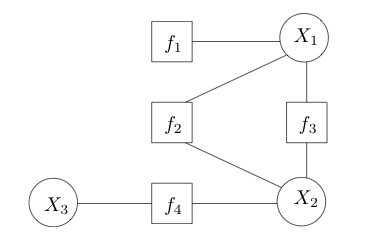
\includegraphics[scale=1]{../bilder/Factorgraph.jpg}
\caption{Beispielfactorgraph}
\label{fig:factorgraph}
\end{figure}
Jede Factornode ist mit den zugehörigen Variablenodes verbunden. Man kann noch erkennen, dass es im Graphen einen Zyklus gibt. Das liegt daran, dass sowohl $f_2$, also auch $f_3$ die Argumente $X_1, X_2$ haben. Da sich beide Faktoren sozusagen aus den selben Argumenten zusammensetzen lassen, kann man diese beiden Faktoren auch zu einem zusammenfassen und der Graph wird zu einem Baum. Das ist relevant, da message passing algorithmen exakt auf Trees funktionieren, während sie für Graphen mit Zyklen nur Approximationen liefern. 

\subsection{Graphen zu Faktorgraphen}
In einem Bsp-paper wird zu einem normalen ungerichteten Graphen ein Factorgraph assoziiert, indem für jeden Knoten ein factor-Knoten gesetzt wird und in jede Kante ein Variableknoten, welcher dann mit zwei Kanten zwischen den factor-Knoten wieder verbunden wird. 

\section{Zustandssumme}
Die ZS ist ein Maß für das Volumen, das ein System im Phasenraum einnimmt.
Vom mikrokanonischen Ensemble ausgehend ist sie eine Funktion der Temperatur $T$ sowie der Mikrozustandsenergien $E_1, E_2, \dots$, welche durch andere thermodynamische Größen ($V$,$N$, etc.) bestimmt werden. Die ZS spielt die Rolle der Normalisierungskonstante und ist nicht abhängig von einem Mikrozustand. Sie sorgt also dafür, dass sich die Wahrscheinlichkeiten $P_s = \frac{1}{Z}e^{-\beta E_s}$ dafür, dass sich das System im Mikrozustand $s$ befindet zu 1 aufsummieren. \\
In the canonical and grand-canonical ensembles the meaning of the partition function remains the same, but since energy is not anymore fixed the expression is going to change.

\section{Survey Propagation}
\subsection{Cluster}
Am Beispiel von min. VC ist ein Cluster eine Zusammenfassung von min. VC die sich nur durch eine kleine Zahl von Änderungen (von Knotenzuständen?) unterscheiden. Dabei gehts aber immer um den selben Graphen.

\subsection{states pro Cluster und Cavity Graph}
Ich sage, ein Knoten hat in einem bestimmten Cluster von ähnlichen min. VC zB den Wert 0, wenn er in keinem min. VC des Clusters gecovert wird.
Wenn ich einen einzelnen Graphen habe und habe dazu den cavity graphen $G_i$ bei welchem für alle Nachbarn von $i$ gilt, dass sie in $G_i$ immer in allen min. VC gecovert sind, dann kann ich für $i$ sagen, dass ich ihn im kompletten Graphen gleich Null setzen kann, da ein min. VC vom cavity graphen so auch eins von $G$ ist.\\\\
Unter der Annahme, dass die Aussagen in diese Richtung gemacht werden (von cavity graph wird auf kompletten Graph gefolgert), kann man dann für ein Cluster folgendes sagen:
Wann wird ein Knoten $i$ im Cluster auf 0 gesetzt? Statt eine Aussage über alle min. VC des Graphen zu machen, schaut man sich hier ja nur die min. VC eines Clusters an.
Siehe Frage \ref{subsec:cluster_frage}
%Das geht meiner Meinung nach nur, wenn für jede die obige Aussage gilt, dass in den cavity graphen immer jeweils alle Nachbarn auf 1 gesetzt sind. Wie überträgt sich das jetzt auf eine Gesamtaussage für das Cluster?


\section{Fragen}
\subsection{Offen: Warum kann man die ZS rekursiv zusammenmultiplizieren (im Vorlesung 13 Optimierungsalgorithmen)}

\subsection{Offen: Wie lässt sich die Berechnung der ZS auf den ER-Graph übertragen, oder auch: Was bedeutet es, die ZS für einen Knoten auszurechnen (Vorl 13 Opti.)}

\subsection{Offen: Zu Cavity graphen und min VC}
Wenn ich einen Knoten $i$ habe und für seinen Cavity-Graphen ein min. VC ausrechne und dabei rauskommt, dass ein Nachbarknoten $j_0 \in N(i)$ in keinem min VC des Cavitygraphen $G_i$ vorkommt, bedeutet das ja, dass dessen Nachbarn (außer $i$) in jedem min VC von $G_i$ vorkommen müssen.\\
Jetzt die Frage: Warum gilt für alle Nachbarn $k \in N(j_0) \setminus \{i\}$, dass $\pi_{k|j_0} > 0$ ist? \\
\textit{Wenn klar ist, dass es ein minimales VC des neuen Graphen ohne $j_0$ geben muss bei welchem alle Nachbarn $k$ gecovert sind, wäre die Aussage schon bewiesen. Klar ist, dass wenn es ein solches min VC gibt, dass dieses auch ein min VC des Graphen mit $j_0$ wäre, da alle Kanten die zu $j_0$ führen automatisch abgedeckt wären. Aber gilt diese Folgerung auch andersrum?\\
Ein anderer Ansatz wäre zu überlegen, ob jeder Nachbar $k$ individuell mindestens in einem min VC vom neuen Graphen vorkommen muss.\\
Vielleicht muss ich die Unabhängigkeit noch mehr in Betracht ziehen?}\\
\\
%Alex meinte jetzt, dass das irgendwie schon durch den Anspruch an globale minimale VC des gesamten Graphen begründet sei, aber das finde ich komisch, da das vorher noch nie ein Thema war und ich dachte, dass der cavity graph sich seine min VC selber bauen darf.
Alex meinte, dass die Begründung eher aus der anderen Richtung kommt: ``Das `implies' soll ausdrücken was die Voraussetzungen dafür sind, dass man $j_0=0$ setzen darf.'' Also nach dem Motto: Unter welchen Umständen kann ich $j_0=0$ setzen. Wenn es so ist, ist das sehr verwirrend geschrieben. 

\subsection{Offen: selbes Thema}
Er schreibt im Abschnitt über SP, dass ein Knoten im Jokerstate exakt einen Nachbarknoten hat, der im Cavitygraphen den State 0 hat, also nie gecovert wird in min. VC des $G_i$. Diese Aussage gilt für einen Graphen, der aus Vier knoten besteht, welche als Linie verbunden sind, denn nehme ich zB den rechtesten Knoten raus, dann kommt dessen Nachbar in keinem min VC von $G_i$ vor. Wenn ich jedoch einen vollständigen Graphen aus drei Knoten nehme, kommen immer zwei in einem min. VC vor, dh alle haben den Jokerstate, aber wenn ich dann einen rausnehme, bleiben zwei verbundene übrig, bei welchen die Aussage scheitert, da ich egal welchen ich nehme ein min VC habe und es keinen Nachbarn gibt, welcher in keinem min VC des $G_i$ vorkommt.\\
Die Aussage ist also nicht allgemein gültig, aber vielleicht für Graphen die Trees / treelike sind? 
Ich muss die Aussage auch nochmal aus dem Punkt betrachten, dass das Zustände sind, die pro Cluster gelten, also zB state 1 sagt aus, dass der Knoten in allen min VC pro Cluster vorkommt, also pro Graph in allen min VCs.

Hier ist wieder die Unabhängigkeit ausschlaggebend. Die Aussage trifft nur für Bäume zu.

\subsection{Offen: Cluster und cavity graph}
\label{subsec:cluster_frage}
Wenn ich es so sehe, dass die States Aussagen in Bezug auf die Cluster machen, dann: Warum muss ein Knoten $i$, der in einem Cluster den Wert 0 hat alle Nachbarn in state 1 ODER * haben? Wenn die Aussage anders rum gemacht wird, dann habe ich doch für ein Cluster die selbe Aussage wie für alle Lösungen für ein min. VC eines Graphen, nämlich dass ich einen Knoten nur dann auf Null setzten kann, wenn im Cavity graph immer alle Nachbarn auf 1 gesetzt sind oder?

Ja, aber hier ist wieder die Unabhängigkeit essentiell. Da es min VC gibt in denen Nachbarn mit Jokerstate gecovert sind, nehme ich mir da die unabhängig sind genau solche damit ich meinen neuen Knoten einfach dazunehmen kann ohne weitere Knoten covern zu müssen.

\end{document}